\documentclass[sigconf]{acmart}
% The preceding line is only needed to identify funding in the first footnote. If that is unneeded, please comment it out.
% On windows run updmap
\usepackage{amsmath,amsfonts}
\usepackage{algorithmic}
\usepackage{graphicx}
\usepackage{textcomp}
\usepackage{listings}
\usepackage{xcolor}
\usepackage{multirow}
\usepackage{dcolumn}
\usepackage{booktabs} 
\usepackage{pifont}  % use /ding{55} for X... /ding{51} for check
\usepackage{url}
\usepackage{hyperref}
\usepackage{adjustbox}
\usepackage{threeparttable}
\usepackage[nameinlink]{cleveref}

\expandafter\newcommand\csname r@tocindent4\endcsname{4in}
\setcounter{secnumdepth}{4}
\setcounter{tocdepth}{4}

\lstset{
language=Java,
basicstyle=\small\ttfamily,			
keywordstyle=\color{blue},
commentstyle=\color{gray},			
stringstyle=\color{black},					
}


\AtBeginDocument{%
  \providecommand\BibTeX{{%
    \normalfont B\kern-0.5em{\scshape i\kern-0.25em b}\kern-0.8em\TeX}}}

% My 'newcommand' for modulo function...
\newcommand{\abs}[1]{\left|#1\right|}


% My 'newcommand' for standard table creation...
\newcommand{\AndreaTable}[3]{\begin{table*}[h!]
\caption{#1}
\centering
\begin{tabular}{#2}
\toprule
#3
\bottomrule
\end{tabular}
\end{table*}
}

% My 'newcommand' for standard table creation...
\newcommand{\equivalenceClassesTable}[2]{
\AndreaTable{#1}{llm{8cm}m{8cm}}{#2}
}


\definecolor{beaublue}{rgb}{0.74, 0.83, 0.9}


\settopmatter{printacmref=false, printccs=false, printfolios =false}
\setcopyright{none} 
\renewcommand\footnotetextcopyrightpermission[1]{}
\acmConference[ISW2 Project A.A. 2019-2020]{ }{September 1, 2020}{ }

\begin{document}

\title{ML Project A.A. 2019-2020}

\author{Andrea Graziani ($0273395$)}
\email{andrea.graziani93@outlook.it}
\affiliation{
  \institution{Università degli Studi di Roma "Tor Vergata"}
  \city{Rome}
  \country{Italy}
}

\keywords{Non-Intrusive Load Monitoring, Time-Series, Walk-Forward (Sliding Window Approach), Hyper-parameters optimization, RNN, LSTM, Early Stopping, Over-Fitting}
\maketitle

\section{Introduction}

\textbf{Non-Intrusive Load Monitoring} (\textbf{NILM}) is the task of estimating the power consumption of each appliance given aggregate consumption. 

Formally, given the \textit{aggregate power consumption} $(x_1, \ldots , x_T )$ from $N$ active appliances, our objective is to deduce the power consumption $(y_1^i, \ldots , y_T^i)$ of appliance $i = 1, \ldots, N$, such that at time $t = 1, \ldots, T$.

The aggregate power consumption $x_t$ at time $t$ is given by the sum of the power consumption of all the known appliances plus a noise term $\varepsilon_t$, that is:

\begin{equation}
x_t = \sum_{i = 1}^N y^i_t + \varepsilon_t
\end{equation}

\section{Data-set}

According to project specification, our data-set includes all observations, regarding the aggregate power consumption, from \textit{2019-01-01 00:00:00} to \textit{2019-03-14 23:59:59}.

A very important characteristic of our data-set it that it contains \textbf{time series} data, where the time of each instance, containing the attribute value regarding power consumption, is given by a \textit{timestamp} attribute; thus our data-set represents a sequence of \textit{discrete-time data} \citep{FalessiDataMining}. All data are listed in time order.

The \textit{sampling frequency}, i.e. the number of sampling points per unit time, is equal to $1$ Hz.

\section{Pre-processing}

In this section, we will describe how we have \textbf{pre-processed} our data before to use our neural network.

Our pre-processing activity is made up of following three step:

\begin{itemize}
\item \textit{Missing data points management}
\item \textit{Standardization}
\item \textit{Feature extraction}
\end{itemize}

\subsection{Missing data points management}

To check the existing of missing values inside aforementioned range, we have built a function called \texttt{manage\_\-mis\-sing\-\_time\_se\-ries\-\_re\-cords}, which detected exactly $224692$ missing data points. 

First of all, to manage missing data, we have filled all the "\textit{holes}" inside our data-set with \texttt{NaN} values. 

Finally, all \texttt{NaN} values was filled via \textit{linear interpolation,} exploiting \texttt{pan\-das\-.Series\-.interpolate}\footnote{\url{pandas.Series.interpolate}} function.

\subsection{Standardization}

Since the range of values of raw data varies widely, we have applied a \textbf{feature scaling} method, according to which all attributes values must to lie in a fixed range \cite{FalessiDataMining}. 

Scientific literature reports that feature scaling techniques are able to accelerate deep network training \cite{Normalization}\cite{FalessiDataMining}.

To be more precise, we used a technique called \textbf{standardization} according to which, after calculating the statistical mean $\mu$ and standard deviation $\sigma$ of attribute values, we subtracted the mean from each value and divide the result by the standard deviation \cite{FalessiDataMining}. Here is the formula for standardization:

\begin{equation}
X' = \dfrac{X - \mu}{\sigma}
\end{equation}

From an implementation point of view, standardization task was performed using  \texttt{RawDataPreprocessor} python class.

To be more precise, we have tried another approach, called \textit{normalization}, which is applied by dividing all values by the maximum value encountered or by subtracting the minimum value and dividing by the range between the maximum and minimum values. However, our trials showed that normalization reduce our neural network performance on test set, therefore this method was been discarded

\subsection{Feature extraction}

Finally, inspired by \citet{meaninpiu}'s report, we have performed a \textbf{feature extraction} activity according to which we built some derived, informative and non-redundant values from our raw data in order to facilitate the subsequent learning and generalization steps.

Precisely, for every $240$\footnote{This value was been heuristically chosen according to our neural network performance on test set.} instances we have calculate $3$ statistical features, that is \textit{mean} values, \textit{minimum} and \textit{maximum} values, adding them to our dataset. This task was performed by \texttt{featu\-res\_extra\-ction} function. 

Our trials showed that adding this activity has improved slightly our neural network performance on test set. 

\section{The Validation Technique}

When working with deep learning, it is vital to have separate \textit{training}, \textit{test}, and \textit{validation} sets. How to identify them?

In order to take into account the time-sensitiveness of our data, we need a \textbf{validation technique}, that is a \textit{technique which defines a specific way to split available data in train, validation and test sets}, capable \textbf{to preserve the temporal order of data}, preventing for example that the testing set contains data antecedent to the training set. These techniques are generally called \textit{time-series} and \textbf{must} be used when the data is time-sensitive \cite{Falessi}.

Therefore, since traditional methods of validation and cross-vali\-da\-tion are unusable in our context, during our project development, we have adopted a widely used time-series technique called \textbf{Walk-Forward} with \textbf{Sliding Window Approach}.

Using this approach, is possible to train our model excluding both any future data including those which are too far in the past too \cite{Falessi}.

\begin{figure}
  
  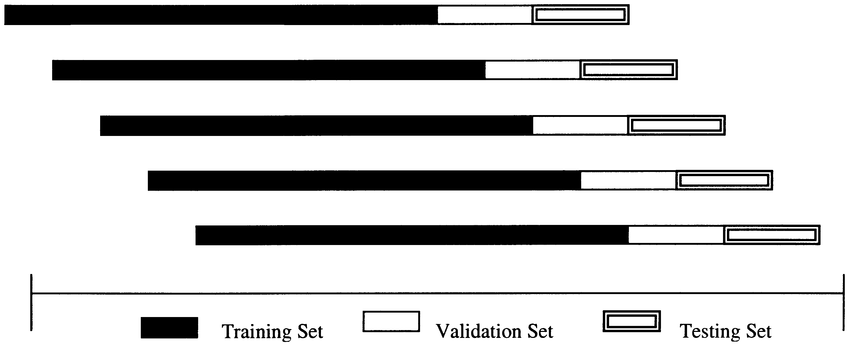
\includegraphics[width=250pt]{walk.png}
  \caption{Walk-forward's scheme used to divide each whole data set into several overlapping training–validation-test sets.
  \label{figureddd}
}
\end{figure}

To be more precise, we have adopted the walk-forward scheme proposed by both \citet{WALK1} and \citet{WALK2} according to which we have divided  whole-data set into overlapping training–validation–testing sets in order to the testing set follows validation set which, in turn, follows training set, respecting temporal order of data. This scheme is shown in figure \ref{figureddd}.

Since, according to project specification, all observations, belonging to \textit{final} test set regarding the temporal range from \textit{2019-03-15 00:00:00} to \textit{2019-03-31 23:59:59}, taking into account the sampling frequency of $1$ Hz, are exactly $1468800$, corresponding to exactly $17$ days of data, according to our scheme each training–validation–testing is made up of as follows:
\begin{itemize}
\item $1468800$ instances for test set ($17$ days).
\item $1468800$ instances for validation set ($17$ days).
\item $2937600$ instances for training set ($34$ days).
\end{itemize}

In other words, each training–validation–testing sets include a total of $5875200$ ($68$ days) instances corresponding to exactly $64$ days of data. 

Finally, we have decided that each training–validation–testing set is moved forward through the time series by $950400$ instances ($11$ days); in this way, we are able to include the final test set during the last iteration of walk-forward scheme.

The main disadvantage of that scheme are the frequent \textbf{retraining} steps which we have to perform as new data becomes available. Despite the scheme is more \textit{time consuming}, it allow us to adapt more quickly to the change of power consumption over the time\cite{WALK1}\cite{WALK2}.

From an implementation point of view, aforementioned validation technique is performed using \texttt{Sliding\-Window\-Walk\-Forward} class.

\section{Neural Network Architecture}

In order to resolve the NILM problem, we have exploited so-called \textbf{recurrent neural networks} (\textbf{RNN}).

We have adopted this kind of network because time series data, such as our data-set, containing aggregate power consumptions, exhibit a dependence on past data, called the \textit{secular trend}\cite{DeepKeras}. In other words, it is said that time series data tend to exhibit a significant \textit{autocorrelation}, which means that a data point value at time $t+1$ are quite likely close to data point value at time $t$.  

RNN networks incorporate this dependence by having a \textit{hidden state}, or \textit{memory}, which makes them prime candidates for tackling learning problems involving sequences of data, such as time series data\cite{DeepKeras}\cite{FalessiDataMining}.

\subsection{A brief digression about RNN}

Formally, the value of the hidden state at any point in time is a function of the value of the hidden state at the previous time step and the value of the input at the current time step, that is:

\begin{equation}
h_t = \Phi(h_{t-1},x_t)
\end{equation}

where $h_t$ and $h_{t-1}$ are the values of the hidden states at the time steps $t$ and $t-1$ respectively, and $x_t$ is the
value of the input at time $t$ \cite{DeepKeras}.

To be precise, to compute the internal state $h_t$, using an activation functions $act()$, we have to compute the sum of the product of the weight matrix $W$ and the hidden state $h_{t-1}$ at time $t-1$ and the product of the weight matrix $U$ and the input $x_t$ at time $t$, that is \cite{DeepKeras}\cite{FalessiDataMining}:

\begin{equation}
h_t = act(Wh_{t-1} + Ux_t)
\end{equation}

Generally, $tanh$ is the most used activation function because its second derivative decaying very slowly to zero, which help to combat so-called \textit{vanishing gradient problem}, that is the problem according to which, for several reasons occurring during back-propagation, the gradient can very easily either diminish to zero or explode to infinity \cite{DeepKeras}\cite{FalessiDataMining}\cite{NILMOTHER}.  

The output vector $y_t$ at time $t$ is the product of the weight matrix $V$ and the hidden state $h_t$, using an activation function, generally a \textit{softmax}\cite{DeepKeras}\cite{FalessiDataMining}:

\begin{equation}
y_t = act(Vh_t)
\end{equation}

Finally just like traditional neural networks, training the \textbf{RNN} also involves \textit{back-propagation}. The difference in this case is that since the parameters are shared by all time steps, the gradient at each output depends not only on the current time step, but also on the previous ones. This process is called \textbf{back-propagation through time} (\textbf{BPTT}) \cite{NILMOTHER}\cite{DeepKeras}. 

\subsection{Our implementation}

Fortunately \texttt{Keras} provides the \texttt{SimpleRNN} recurrent layer that incorporates all the logic we have seen so far. 

Despite the \texttt{SimpleRNN} layer performs well, we have decided to adopt so-called \textbf{LSTM} (\textbf{Long short term memory}) neural network, a variant of RNN capable of learning long term dependencies and specifically created to address the vanishing gradient problem \cite{DeepKeras}\cite{FalessiDataMining}\cite{NILMOTHER}. 

The exact configuration of our regression neural network is as follows:

\begin{itemize}
\item \textbf{Conv1D}, \textsc{convolutional layer} with $F$ filters, kernel size $K$, stride $1$, and \textsc{ReLU} activation function.

\item \textbf{LSTM}, \textsc{Long short term memory} with $H$ units.

\item \textbf{Dense}, that is a \textsc{fully connected layer} with $D$ units and \textsc{ReLU} activation function.

\item \textbf{Dense}, that is a \textsc{fully connected layer} with $D/2$ units and \textsc{ReLU} activation function.

\item \textbf{Dense}, that is a \textsc{fully connected layer} with $D/4$ units and \textsc{ReLU} activation function.

\item \textbf{Dense}, that is a \textsc{fully connected layer} with $1$ units and \textsc{linear} activation function.
\end{itemize}

In principal, the convolutional layer was not expected, however our trials show that the addition of a convolution layer
slightly increases performance on test set.

\section{Hyper-parameters optimization}

As known, best performance on a test set is achieved by adjusting the value of several \textbf{hyper-parameters} to suit the characteristics of data. 

First of all, we remember that, during hyper-parameters optimization, it is very important \textit{not to use performance on the test data to choose best values for hyper-parameters}. This is because peeking at the test data to make choices automatically introduces optimistic bias in the performance score obtained from this same data. Performance on future new data will very likely be worse than the estimate \cite{FalessiDataMining}.

In our project, hyper-parameters optimization regards following elements:

\begin{itemize}
\item The number of filters ($F$).
\item The size of each kernel ($K$).
\item The number of neurons of \textit{Dense} layer ($D$).
\item The number of neurons in the recurrent layer ($H$)
\end{itemize}

To do hyper-parameters optimization we perform the hyper-parameters optimization scheme proposed by \citet{FalessiDataMining}. 

According to their scheme, we have trained our neural network model several times with different hyper-parameter values using, clearly, the training set, and each of the resulting neural network models is evaluated using the validation set.

Once the hyper-parameters values, that give best performance on the validation set (minimum value of validation loss), have been determined, a \textit{final neural network model is built with that hyper-parameters values} and trained with\textit{both} aforementioned training and validation sets.

As stated by \citet{FalessiDataMining}, omitting data belonging to validation set from final training can reduce performance in the test but, at the same time, this choice can be risky due to over-fitting. The \citet{FalessiDataMining}'s solution is to stop training after the same number of epochs that led to the best validation set performance.

Only after the final model is fixed are we allowed to use the test data to obtain an estimate of the performance of this model on new, unseen data. Basically, the test data can only be used once, to establish the final \textit{Energy Based F1} performance score.

From implementation point of view, hyper-parameters optimization is performed using \texttt{start\_\-hyper\-para\-meters\_\-sele\-ction\-\_phase} function.

\subsection{Early stopping}

Early stopping is employed as a form of regularization to avoid over-fitting since it stops the training when the error on
the validation set starts to grow. 

\section{How to run}

To establish the final \textit{Energy Based F1} performance score on test set regarding the temporal range from \textit{2019-03-15 00:00:00} to \textit{2019-03-31 23:59:59}, is necessary to execute following steps:

\begin{itemize}
\item Open \texttt{Nilm.ipynb} file using \textit{Google Colab}\footnote{\url{colab.research.google.com}}

\item Execute all code inside "\textit{Imports, 'Google Drive' mounting and GPU checking}", "\textit{Project's functions...}" and "\textit{Project's classes...}" sections of the notebook. 

Make sure to mount \textit{Google Drive} on \texttt{/content/drive} directory.

\item Following files \textbf{must} exist on \textit{Google Drive}:
\begin{itemize}
\item \texttt{main\_train.csv}
\item \texttt{fridge\_train.csv}
\item \texttt{dishwasher\_train.csv}
\end{itemize}

\item Following files, regarding test sets, \textbf{must} exist on \textit{Google Drive}:
\begin{itemize}
\item \texttt{main\_test.csv}
\item \texttt{fridge\_test.csv}
\item \texttt{dishwasher\_test.csv}
\end{itemize}

\item Load into current session's main directory following files:
\begin{itemize}
\item \texttt{dishwasher\_neural\_network.h5}
\item \texttt{fridge\_neural\_network.h5}
\end{itemize}

\item Run all code inside "\textit{Script for final testing...}". The final \textit{Energy Based F1} performance score will be displayed automatically.
\end{itemize}

\bibliographystyle{ACM-Reference-Format}
\bibliography{Bibliography}

\end{document}
\endinput








